% Intended to be compiled with XeLaTeX

\documentclass[11pt,letterpaper]{article}

\usepackage{graphicx}
\usepackage{natbib}
\usepackage{fullpage}
\usepackage{lineno}
\usepackage{multirow}
%\usepackage{wrapfig}
\usepackage{amsmath}
\usepackage{amssymb}
%\usepackage{sidecap}
\usepackage{hyperref}
\usepackage{bibentry}
\nobibliography*

\begin{document}

\setlength{\parindent}{0mm}
\setlength{\parskip}{0.4cm}

\bibliographystyle{apalike}

%\modulolinenumbers[5]
%\linenumbers

\title{\textbf{GEMINI} Implementation Details}
\author{Matthew D. Zettergren, PhD\\ \texttt{matthew.zettergren@icloud.com}}
\maketitle

\tableofcontents

\pagebreak

\section{GEMINI Model:  Executive Summary}

\textbf{GEMINI:}  The ``\underline{G}eospace \underline{E}nvironment \underline{M}odel for \underline{I}on-\underline{N}eutral \underline{I}nteractions'' is a 3D ionospheric model based on \citet{Zettergren:2012}, that has been applied in wide variety of ionospheric studies (Zettergren, op.\ cit.).  The model uses a tilted dipole \citep{Huba:2000} or Cartesian mesh, and comprises a fluid system of equations \citep{Schunk:1977,Blelly:1993} describing dynamics of the ionospheric plasma, self-consistently coupled to a quasi-static (defined below) treatment of electrical currents. The fluid system is a set of three conservation equations (mass, parallel momentum, and energy) for each ionospheric species \citep[][ Appendix A]{Zettergren:2015}.  Source terms in the continuity equations include photoionization \citet{Solomon:2005,Richards:1994} and impact ionization via integration of the physics-based energetic electron transport model, GLOW \citep{Solomon:2001}.  Efficient semi-empirical methods for energy deposition calculations \citep{Fang:2008} can also be used.  A full set of chemical reactions needed for the E- and F-regions is taken from \citet[][]{Diloy:1996,StMaurice:1998}.

Perpendicular components of the plasma momentum equations in GEMINI are resolved via a quasi-static force balance approximation \citep{Zettergren:2015b}, viz. a static solution is applied but the parameters of the system  (importantly conductivity) are allowed to change in time.  Electric fields are found by enforcing a divergence-free current density, where the current consists of conduction, polarization, and pressure contributions \citep[e.g. as in][]{Kintner:1985}. This approach assumes a leading order electrostatic description supplemented by terms correcting for polarization currents from varying field structures \citep{Mitchell:1985} (i.e. ion inertial effects).  Because the GEMINI solver is inherently (quasi-)static in nature it can be driven from either field-aligned current (FAC) or electric field conditions boundary conditions.  Specifically, the ionospheric electric field is approximated by $\mathbf{E}=-\nabla \Phi$ but current closure solutions include ion inertial effects.  
\begin{figure}
  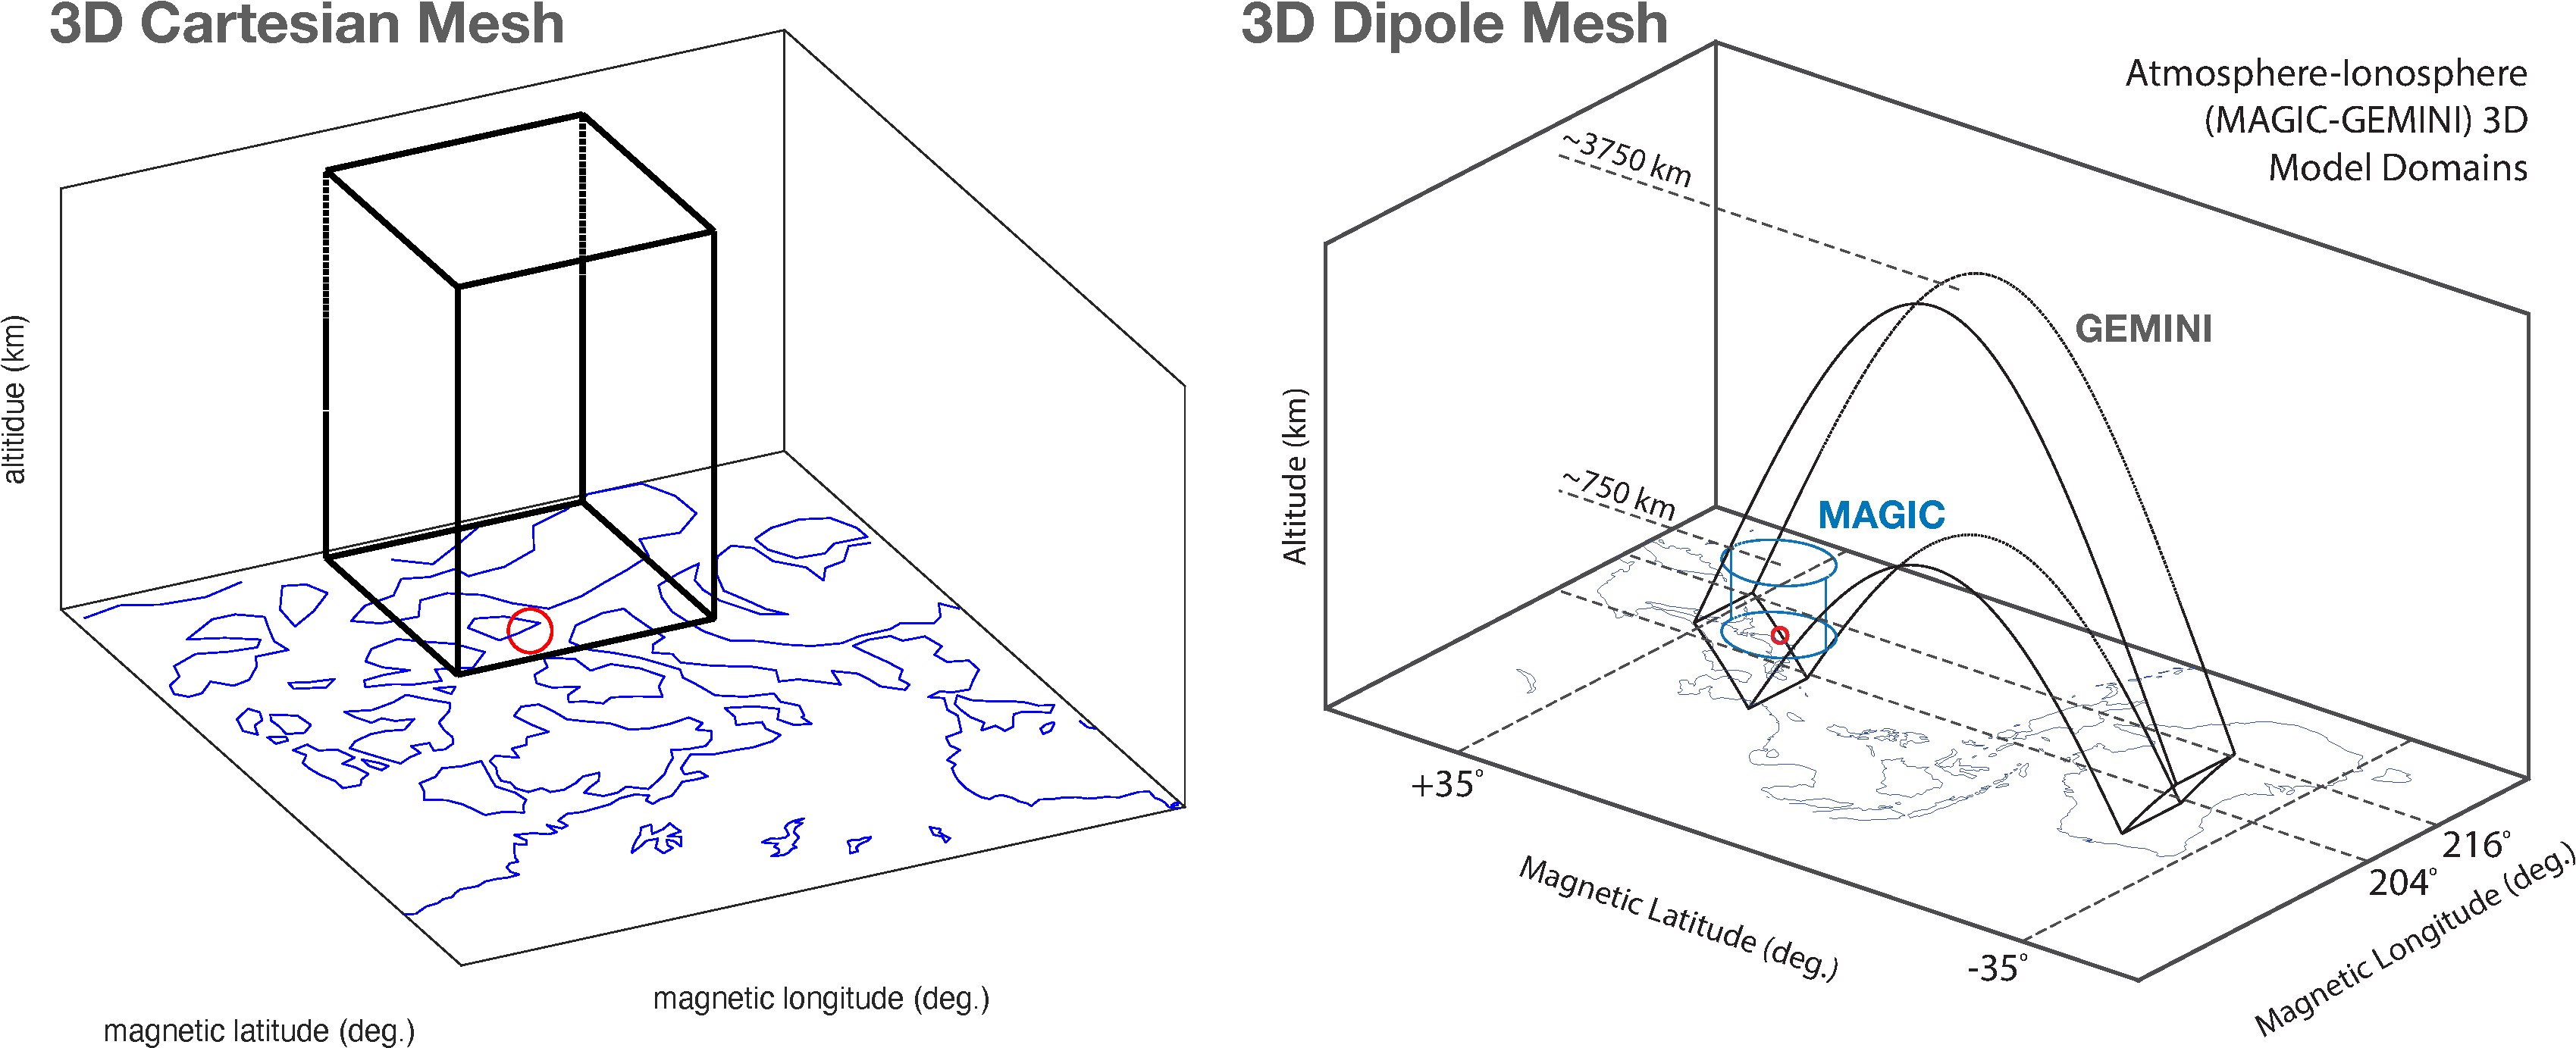
\includegraphics[width=\textwidth]{./figures/GEMINI_mesh-crop.pdf}
  \caption{Examples of commonly used GEMINI mesh configurations: (left) a Cartesian mesh centered near the geomagnetic pole near Resolute Bay Canada, (right) an interhemispheric dipole mesh used with studies of infrasound and gravity wave impacts on the ionosphere.  }
  \label{fig:GEMINI}
\end{figure}

The use of a quasi-static solution notably omits Alfv\'en waves; however, many mesoscale structures are well-described as static \citep[e.g.][]{Lynch:2015}.  Recent reviews suggest that alternating current (AC) Poynting flux is typically reported at lower levels than direct current (DC) Poynting flux, but can be highly variable; the relative importance of these two sources (DC vs. AC) is unknown \citep{Kaeppler:2022}.  Our modeling focuses on the DC input effects (and particle inputs) as we argue this is the only part of the Poynting flux that can feasibly be captured by non-idealized models -- resolving propagation of Alfv\'en waves in a cross-scale (meso-to-large), 3D ionosphere-thermosphere (plasma-neutral coupling) model is computationally infeasible for resolutions and grid extents that we target.   At the very minimum, research suggests that the DC part of the incoming energy and momentum (stress) is a major (perhaps even the largest) contributor and our data-driven methodology permits us to evaluate the extent to which the observations are DC.  As better computational resources and algorithms become available in the future it should be possible to begin to address AC portions of the spectrum, but that is not within the project scope.  

GEMINI presently assumes that the geomagnetic field lines are equipotentials (a particularly good assumption for highly conducting situations likely to accompany precipitation) and employs a field line integration in the equation solved to describe conservation of charge \citep[cf.][Equation 1]{Zettergren:2015}.  Newer versions of GEMINI also include additional current terms needed for high-resolution modeling, like diamagnetic currents and diffusive transport perpendicular to $\mathbf{B}$. 

A comprehensive set of documentation describing the mathematical formulation of the model and some details of numerical solutions is not included here for brevity, but may be found in the \href{https://github.com/gemini3d/gemini-docs}{gemini-docs} repository, specifically at \url{https://github.com/gemini3d/gemini-docs/blob/main/formulation/GEMINI.pdf}.  

\section{GEMINI Model Heritage}

The use of GEMINI for scientific applications is documented in a number of studies and associated refereed journal articles:  
\begin{itemize}
  \item \bibentry{Zettergren:2012}
  \item \bibentry{Zettergren:2013}
  \item \bibentry{Zettergren:2014}
  \item \bibentry{Zettergren:2015}
  \item \bibentry{Zettergren:2015b}
  \item \bibentry{Lynch:2015}
  \item \bibentry{Perry:2015}
  \item \bibentry{Burleigh:2017}
  \item \bibentry{Swoboda:2017}
  \item \bibentry{Zettergren:2017}
  \item \bibentry{Burleigh:2018}
  \item \bibentry{Zettergren:2019}  
  \item \bibentry{Burleigh:2019}  
  \item \bibentry{Deshpande:2019}  
  \item \bibentry{Inchin:2020} 
  \item \bibentry{Spicher:2020}   
  \item \bibentry{Inchin:2021} 
  \item \bibentry{Diaz:2021} 
  \item \bibentry{Clayton:2021} 
  \item \bibentry{Lamarche:2022} 
  \item \bibentry{Burleigh:2022}  
\end{itemize}

These studies encapsulate a wide range of applications of the model from equatorial to low/mid-latitude and high-latitude and a number of studies where the model output has been critically compared against available data in validation exercises.  Additional validation tests not yet published are included in other sections of this document.  

Due to the amount of testing, verification, and validation done as part of the GEMINI's development, the technology readiness level (TRL) of the model is suggested to be TRL6.  



\section{GEMINI Source Code Repositories}

GEMINI is organized into about a dozen repositories ranging from core model numerical parts to scripts that allow one to build all external library dependencies.  To run the code requires two repositories to be built (\texttt{external} and \texttt{gemini3d}) and installed while visualization requires a third, scripting library (either \texttt{mat\_gemini} or \texttt{pygemini}).  

Additionally trees-GEMINI (cf. Section \ref{sec:tG}) supports visualization toolkit output files (vtu) which can be plotted using the open source, 3D visualization software Paraview.  Paraview represents a notable exception to the required visualization back-end scripts; \texttt{vtu} files can be read directly into Paraview using its graphical interface.  

A complete list of gemini repositories and their basic purposes follow (see repository readme files for details).  These are all collected into the \href{https://github.com/gemini3d/}{gemini3d organization} - and ``umbrella'' organization that holds all GEMINI code repositories, documentation, and bug-tracking and includes:  
\begin{itemize}
  \item \href{https://github.com/gemini3d/gemini3d/}{gemini3d} - the core GEMINI fortran, C/C++ code.  
  \item \href{https://github.com/gemini3d/pygemini}{pygemini} - Python front- and back-end scripts for preparing simulation input data and gridding and plotting output.  
  \item \href{https://github.com/gemini3d/pygemini}{mat\_gemini} - MATLAB front- and back-end scripts for preparing simulation input data and gridding and plotting output.  
  \item  \href{https://github.com/gemini3d/gemini-docs}{gemini-docs} - Set of documentation for the model
  \item  \href{https://github.com/gemini3d/gemini-examples}{gemini-examples} - Set of initialization files and scripts for creating different types of simulation setups.    
\end{itemize}



\section{Internal Organization of GEMINI}

Figure \ref{fig:org} shows a top level diagram of GEMINI inputs and coupling with other AIRWaveS models, specifically for the situation where model data are passed through files -- recent advances have made it possible to pass information from MAGIC into GEMINI through memory using the forestclaw mesh management software; however, GEMINI still retains the ability to do coupling through file input/output, which while slower is simpler to use and does not require AMR-related libraries.  
\begin{figure}
  \centering
  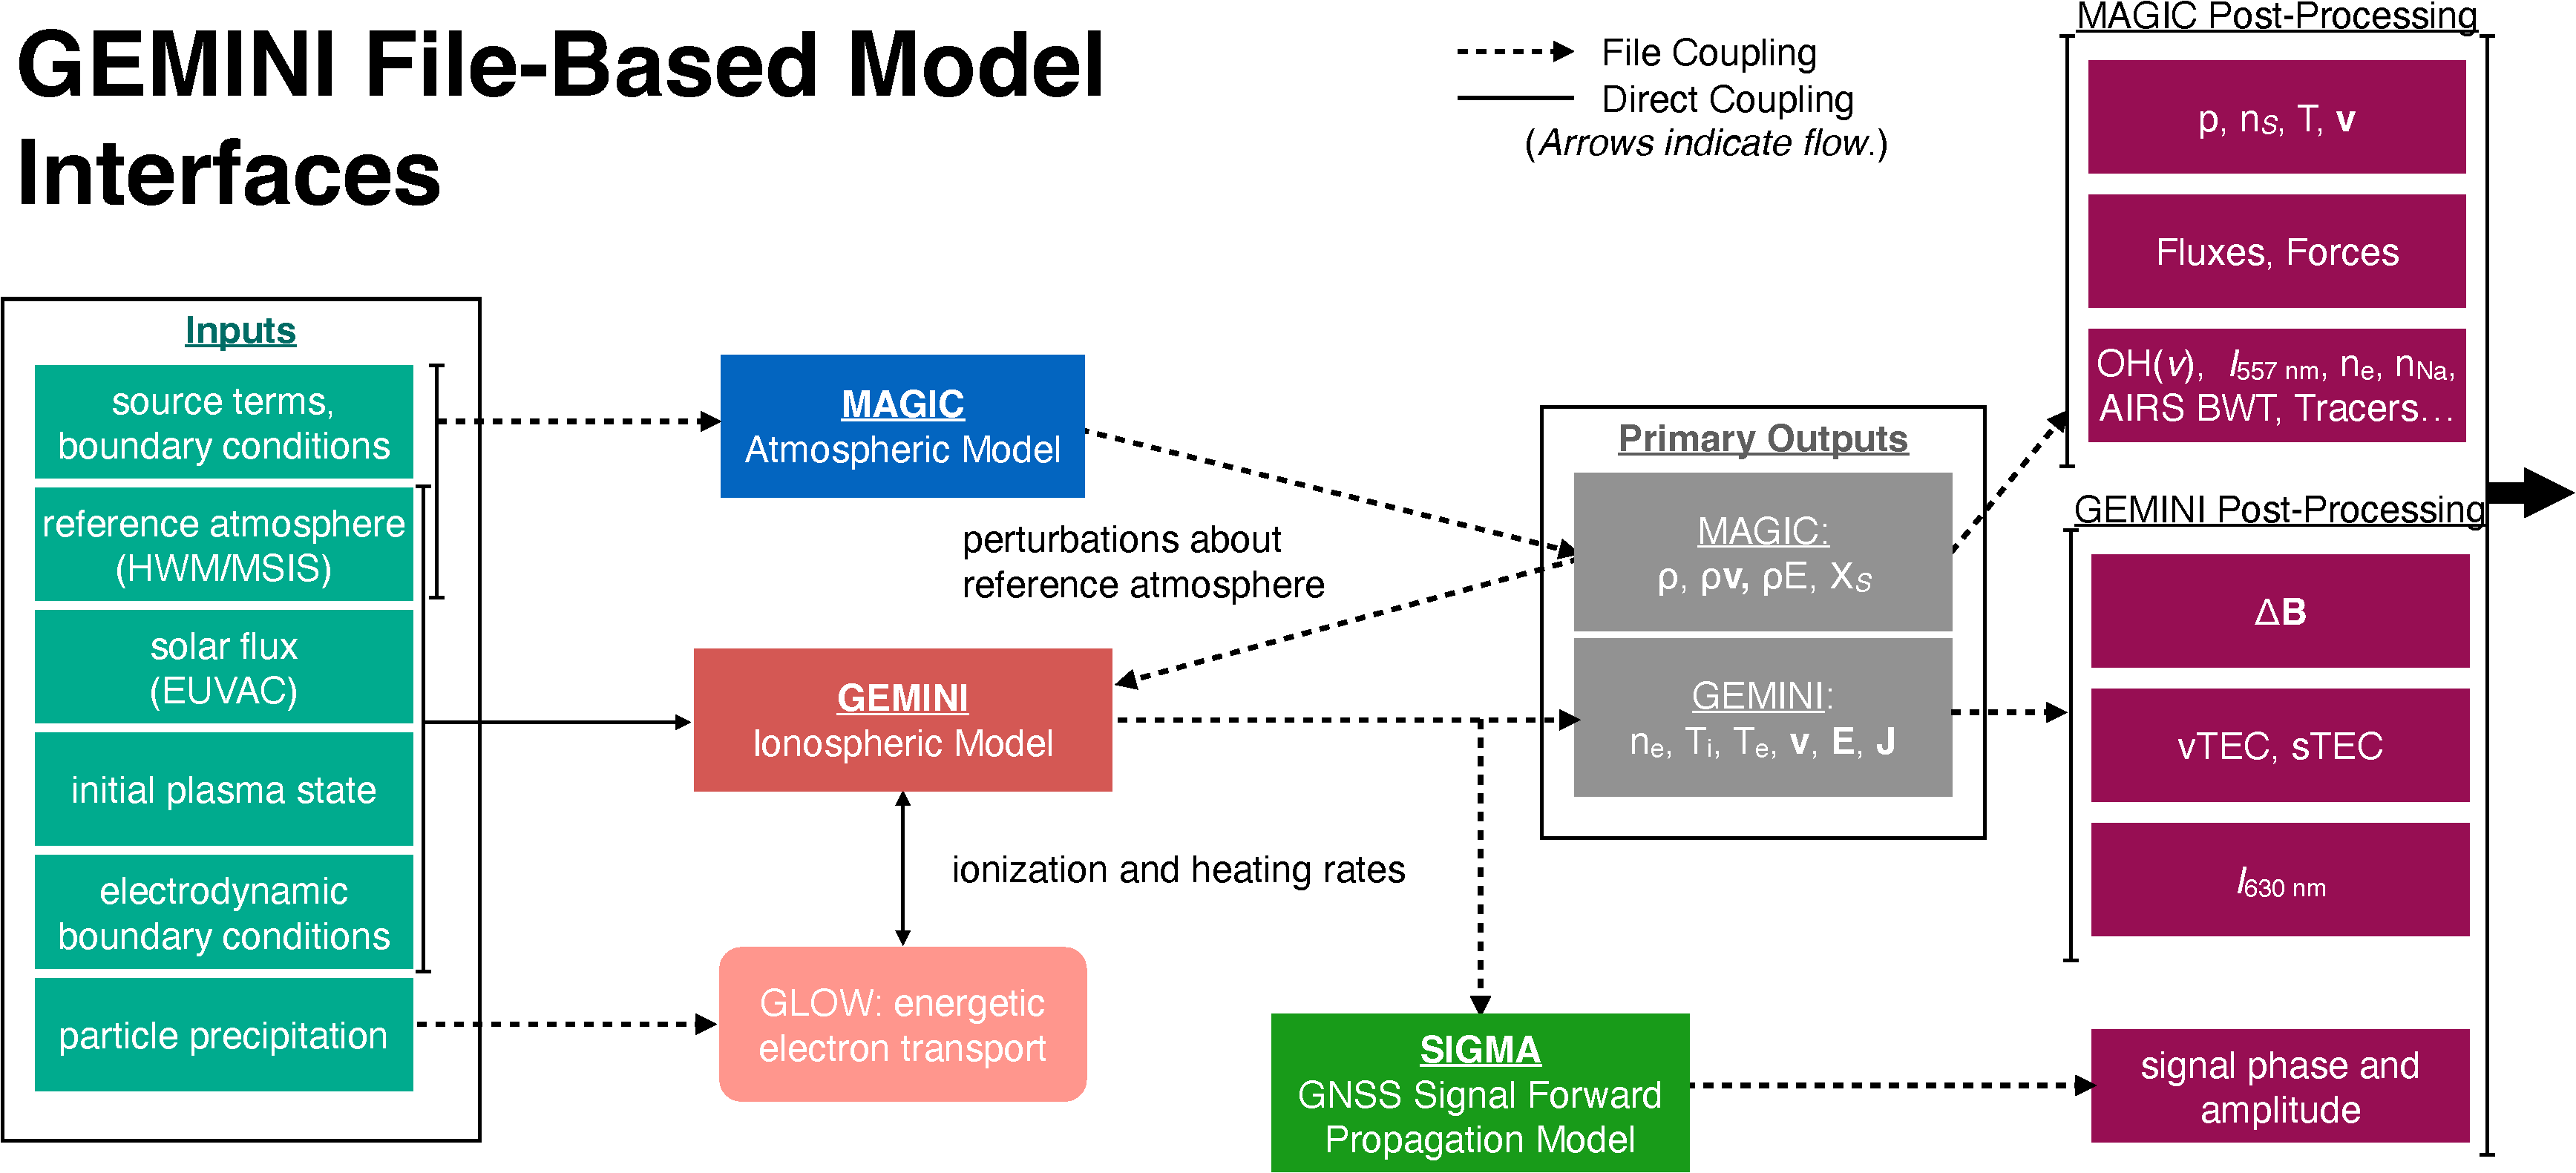
\includegraphics[width=\textwidth]{./figures/GEMINI_org-crop.pdf}
  \caption{GEMINI file-based interfaces and postprocessing.} \label{fig:org}
\end{figure}

The main GEMINI model inputs that need to be provided (through files) are:
\begin{itemize}
  \item Source terms for generating perturbations in the MAGIC model 
  \item Solar fluxes for describing dayside photoionization processes (where relevant)
  \item An initial ionospheric state; this is often generated through an ``equilibrium'' simulation where the model is run for a full day or longer with only solar forcing.  
  \item Boundary conditions for electromagnetic solutions (background electric fields, boundary pottentials and/or field-aligned currents)
  \item Kinetic boundary conditions for specifying high-latitude electron precipitation inputs (as needed)
  \item Reference atmospheres (usually from empirical models)
  \item Atmospheric perturbations from external models (e.g. MAGIC), as required
\end{itemize}
GEMINI provides 3D and time-dependent plasma output parameters including density, drift, and temperature of the 7 main ion species resolved along with electric field and current densities.  Additionally information about magnetic field perturbations and optical intensities (in the case of chemically reactive species) can be computed from the output.  The plasma density fluctuations computed in the model can further be used as input to the SIGMA radio propagation model in order to better-diagnose scintillation and refractive/diffractive effects.  

Core GEMINI model components are implemented in fortran 2008, which interfaces provides for use with C/C++ applications.  Fortran code is organized, from the top-level organizational perspective into modules which encapsulate key numerical functionality.  These are called from the top level \texttt{libgemini} module which provides public interfaces to functionality needed to execute an ionospheric simulation.  
\begin{figure}
  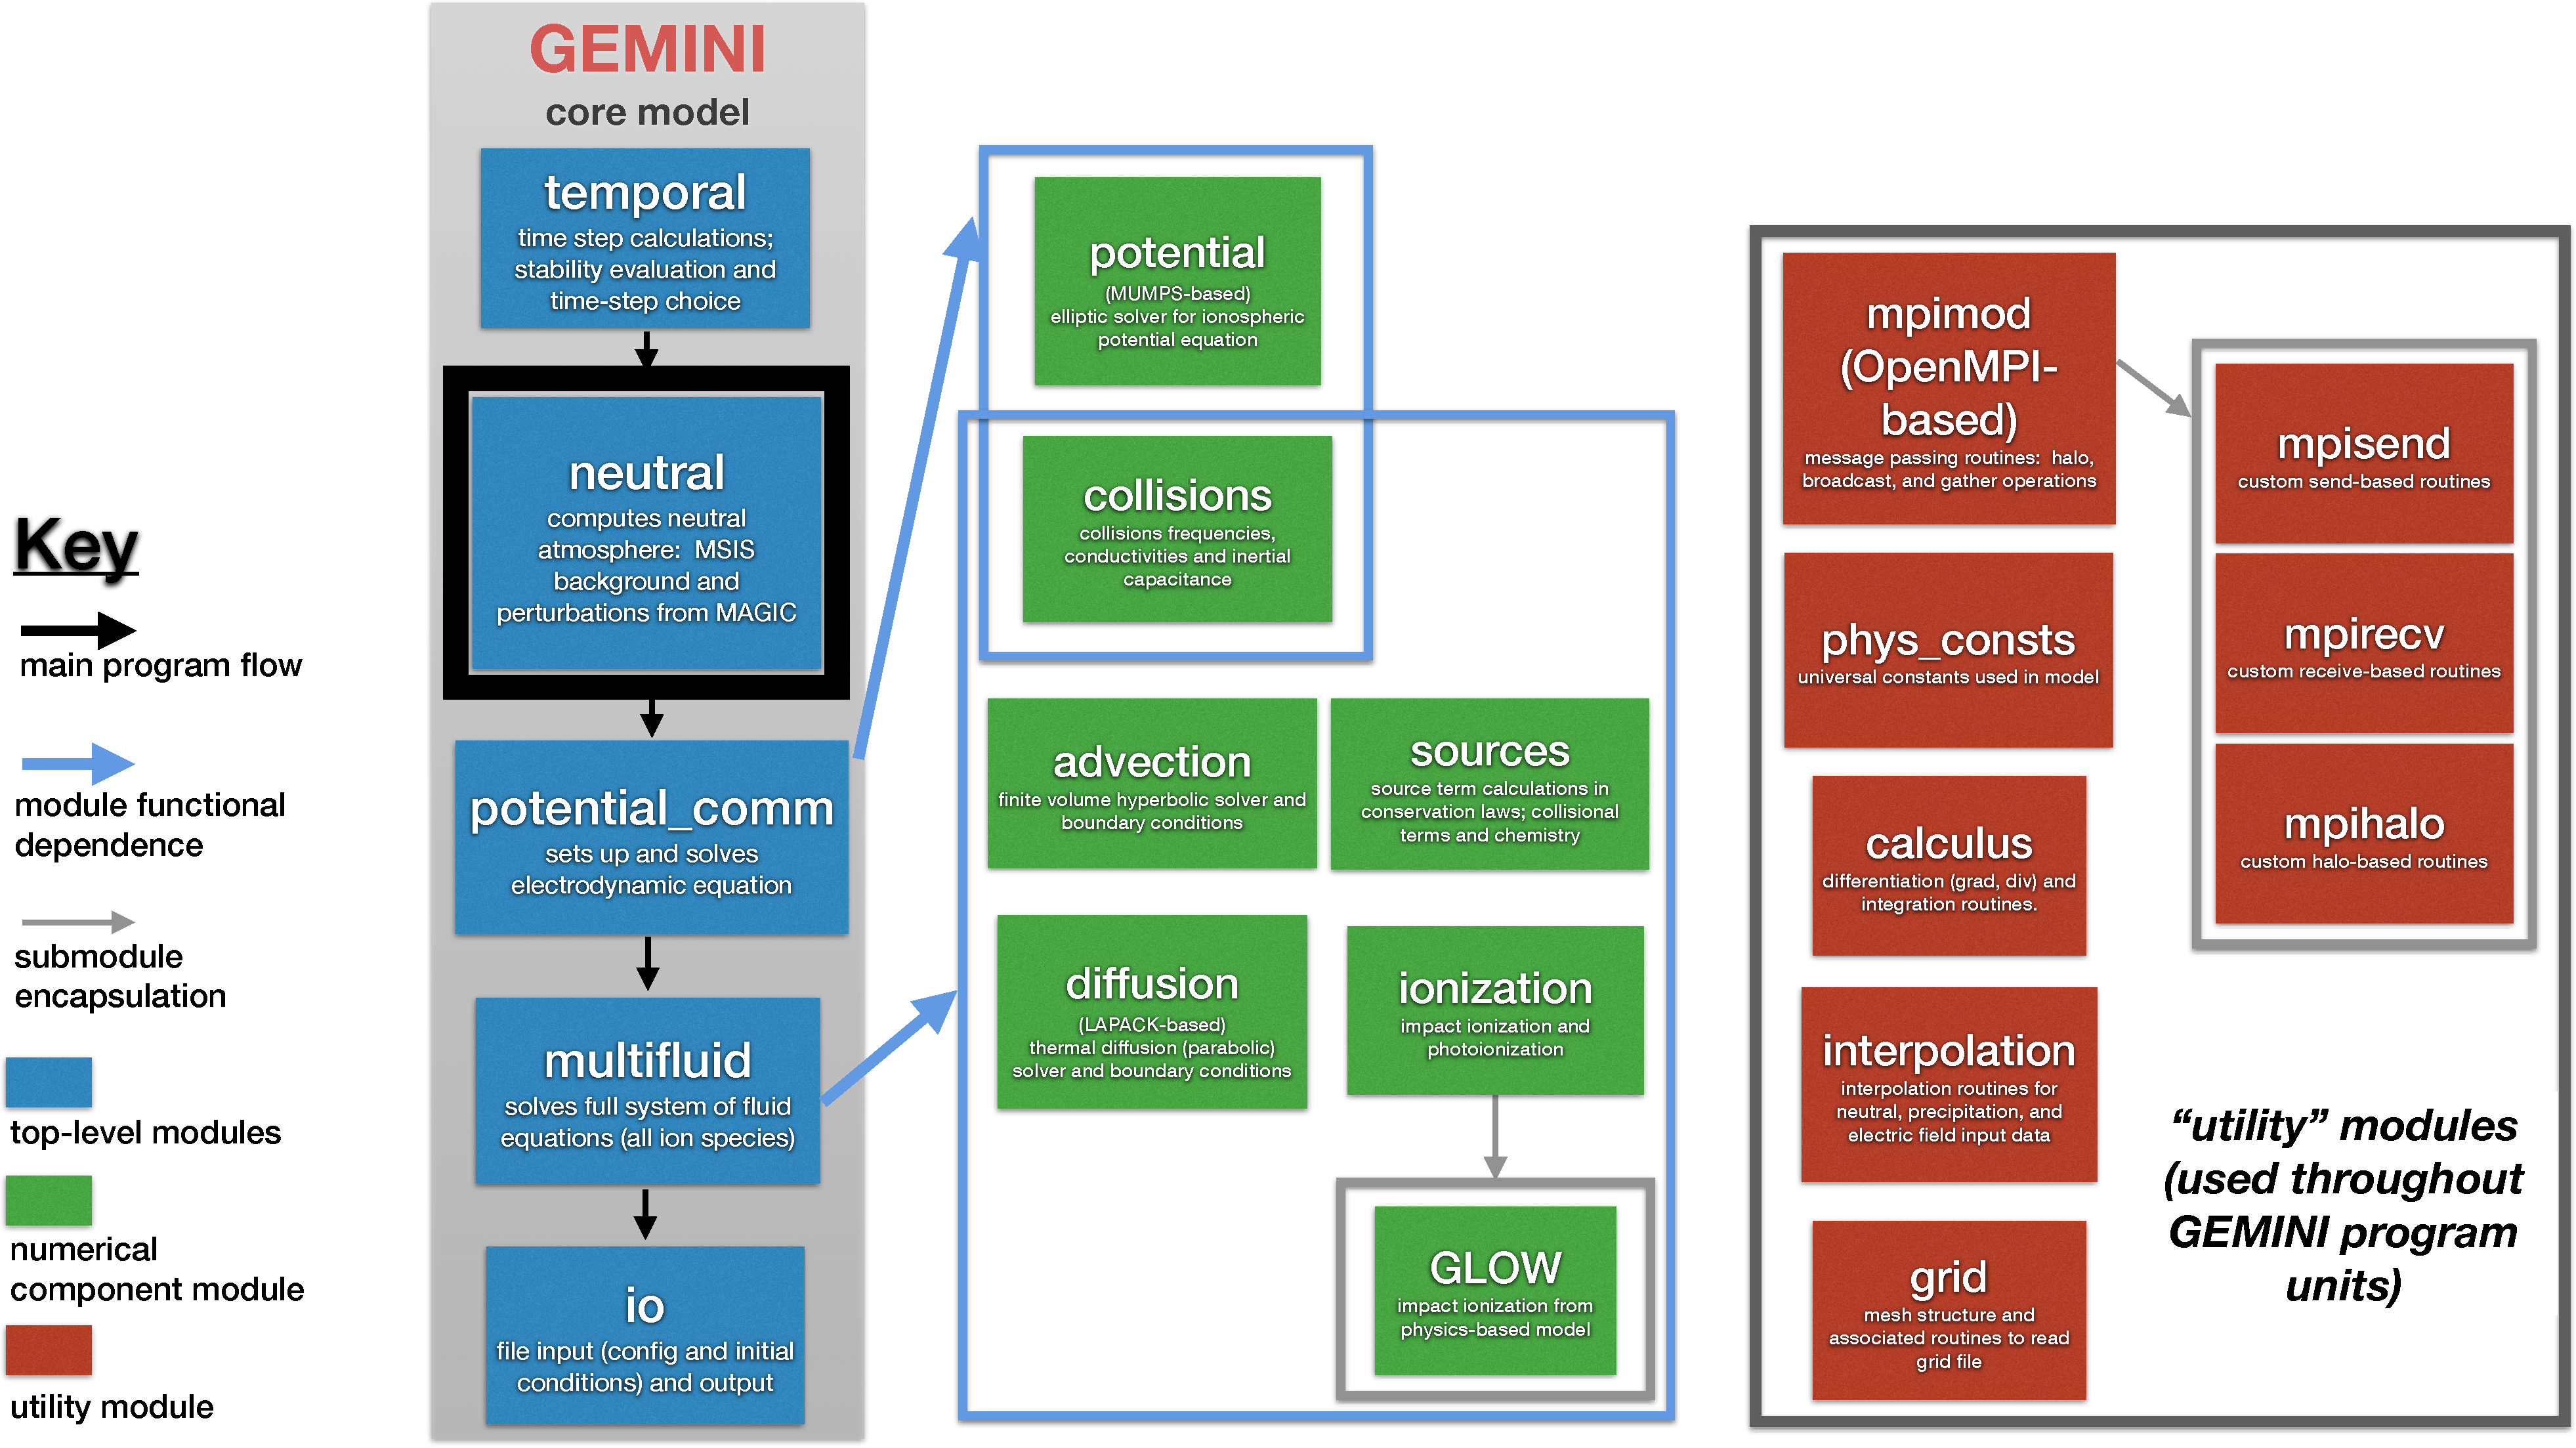
\includegraphics[width=\textwidth]{./figures/modules-crop.pdf}
  \caption{Limited illustration of some of the modules comprising libgemini and the GEMINI ionospheric model.}
  \label{fig:module}
\end{figure}

A complete module listing with all dependencies is almost impossible to represent via a diagram (such information can be obtained from the cmake build files); instead here we illustrate a small subset of these module connexions to illustrate the overall logic to how the modules are organized.  Figure \ref{fig:module} shows the basic flow of the top level programs starting with time step selection and moving through gathering of neutral input data, then solution of electromagnetic equations, plasma transport, and then file output steps.  Some of the module dependencies are shown for electromagnetic and multifluid modules specifically in addition to utility modules required by many (if not most) other modules, e.g. interpolation, grid, and basic calculus operations).  

A detailed description of the neutral module is shown in Figure \ref{fig:neutral} to show the complex internal dependencies of just this single program unit.  This diagram is effectively one layer of abstraction below that shown in Figure \ref{fig:module}.  The neutral modules contains submodules for computing density and temperature (atmos) along with winds (wind) and doing various rotations and transformations to map geographic quantities into geomagnetic.  Likewise there are a number of dependencies on utility routines that provide interpolation, etc., along with external connections needed for message passing communication.  
\begin{figure}
  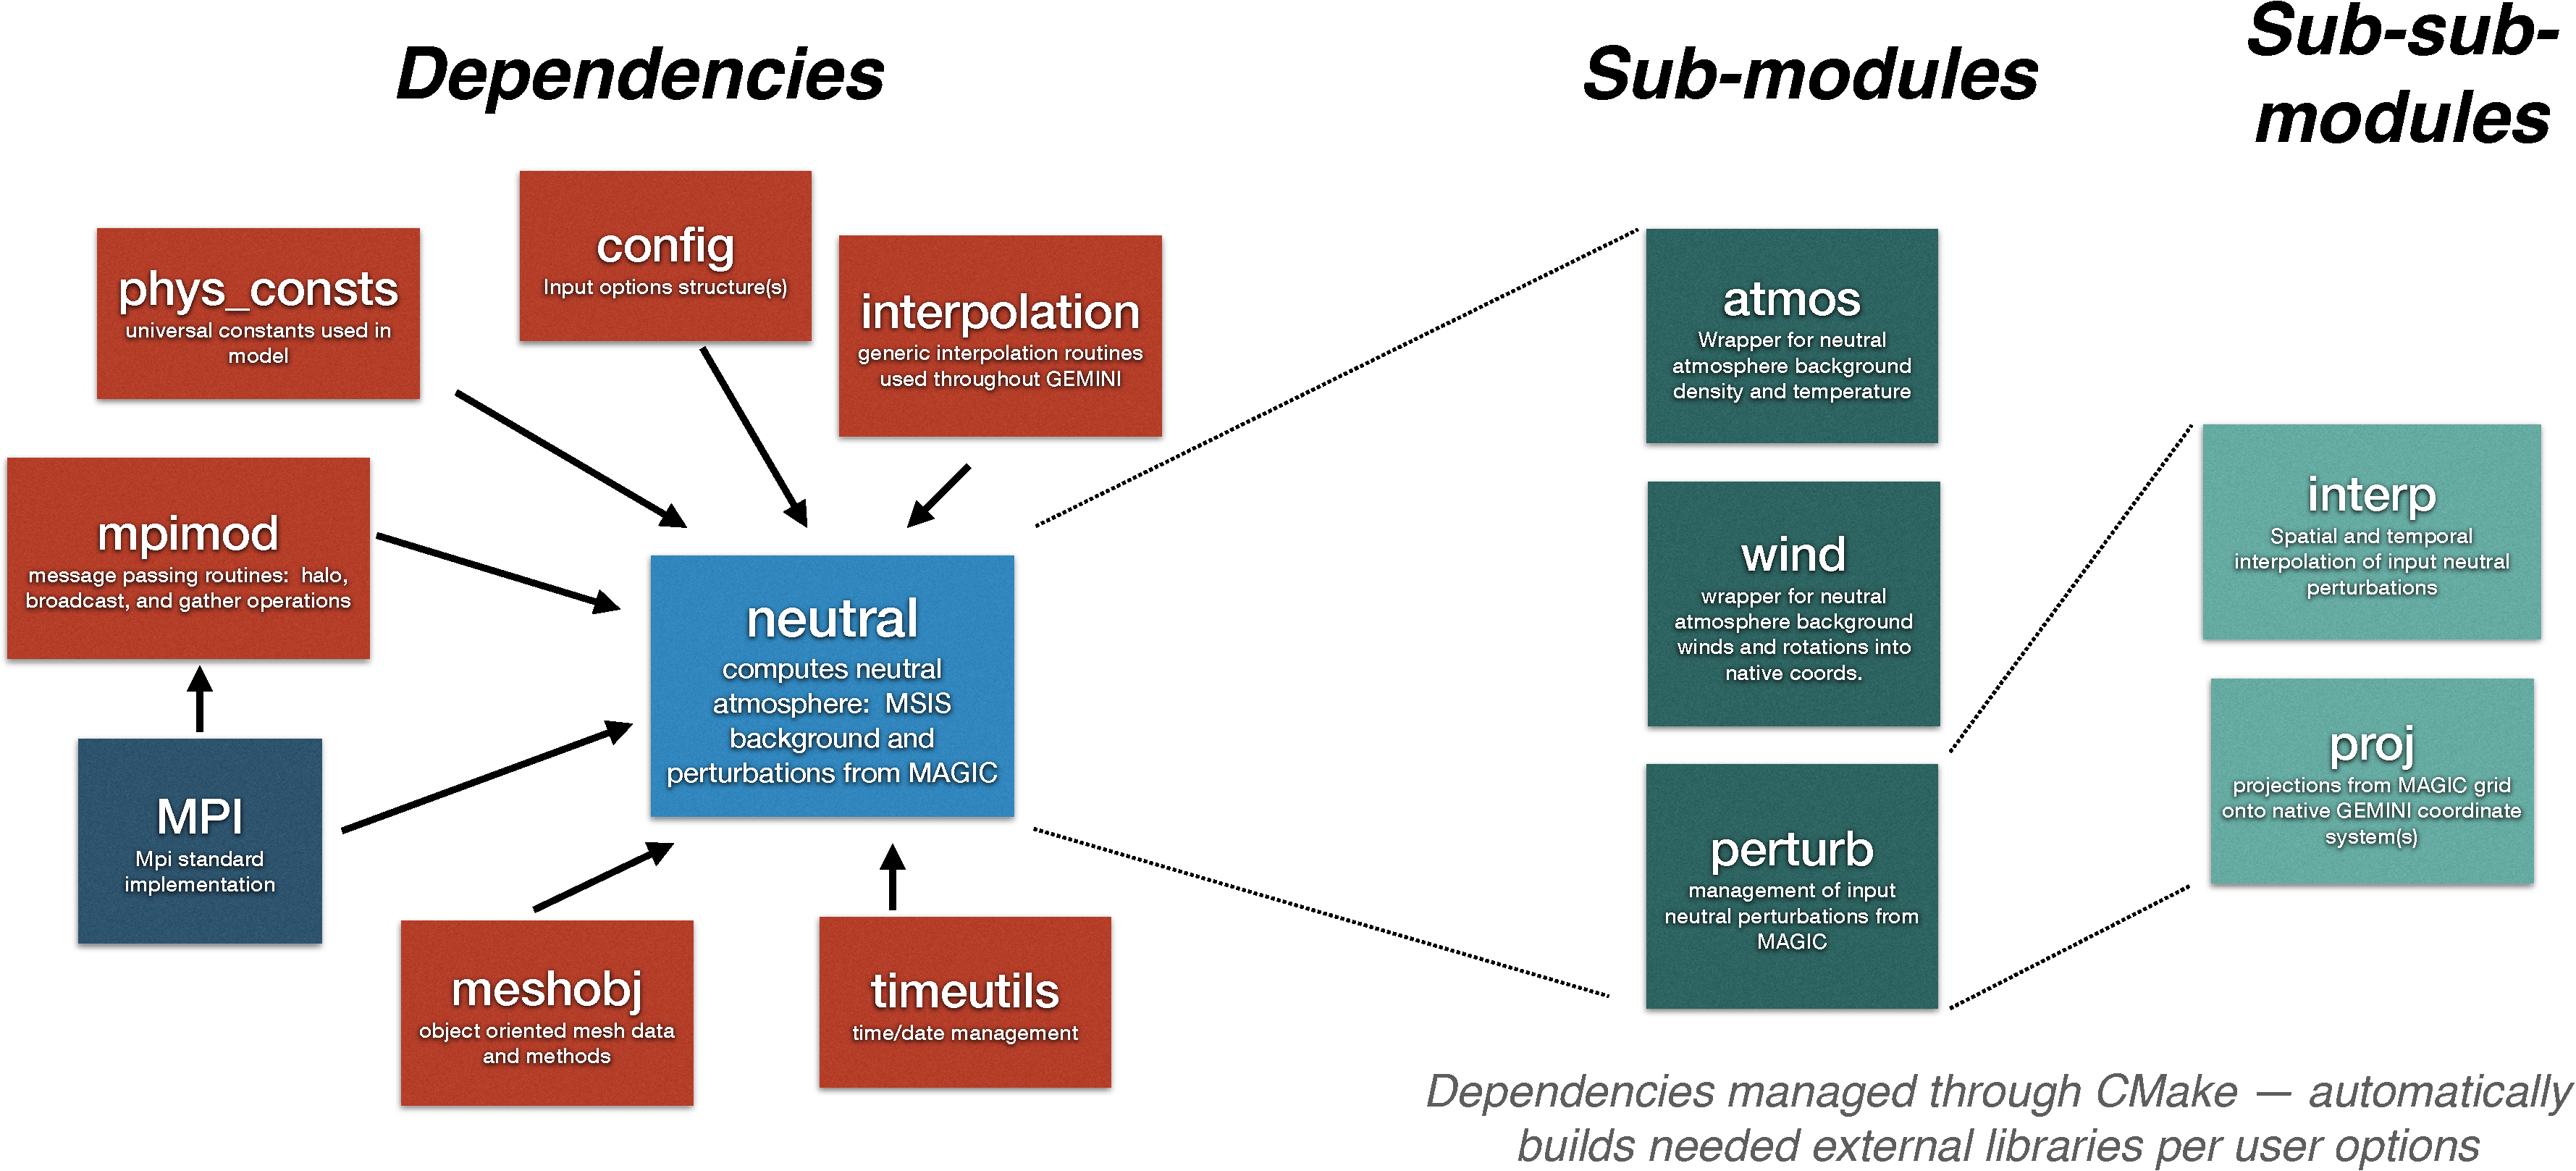
\includegraphics[width=\textwidth]{./figures/neutral-crop.pdf}
  \caption{Diagram for neutral module in GEMINI along with associated submodules and dependencies.}
  \label{fig:neutral}
\end{figure}



\section{Cmake Build System for GEMINI}

\emph{MH - focus on current state and additions made during AIRWaveS}



\section{GEMINI Data Structures}

Until recently data have largely been encapsulated in modules as module global variables that can be accessed from other program units via \emph{use} statements.  While this makes for easy implementation for a number of numerical solutions, it has the issue that there can be only only one set of data per mpi worker (i.e. each worker has one module ``instance'').  To address this issue, it makes sense to encapsulate data and associated procedures using fortran object-oriented capabilities.  These allow us to better organize our data and pass it simply into processing routines along with the necessary feature that one worker can possess multiple data objects, for our purposes  grid and solution data for multiple forestclaw patches.  


\subsection{Mesh Objects}

The use of AMR requires the capability to recompute and reconfigure a mesh arbitrarily during runtime; furthermore, this calculation must not exceed the roughly the computational cost of a typical time step to fully benefit AMR (TA 1.1.2, 1.1.3).  Historically GEMINI meshes had been computed by the MATLAB front-end scripting environment (\texttt{mat\_gemini}).

As part of this project we have also added the ability to compute meshes using \texttt{pygemini}, in case these are needed for any pre- or post-processing tasks.  

Additionally to address needs of dynamic re-meshing the input grid information is handled differently now.  Instead of having the root process read in the grid coordinates, along with all metric factors, unit vectors, and additional information like magnetic field strength, only the coordinate array are passed into the GEMINI core code and then then all other quantities are computed from these internally and by each worker or patch instance of the model.  This effectively parallelizes the computationally expensive parts of the mesh generation, with testing showing a 10x improvements in performance on a single core (when compared against script mesh generation and, on top of that, almost perfect scaling with the number of cores used for the mesh generation.

There is also the potential that AIRWaveS and future related activities may need additional coordinate systems other than dipole or Cartesian.  Thus, during the process of absorbing the mesh generation were into the core GEMINI code we created an object-oriented approach to the organization of mesh data within a given \texttt{mpi} worker (or forestclaw patch).  This approach has benefits of making it relatively clean and easy (from a coding point of view) to adapt new mesh types using different coordinate systems. Additionally these objects can be passed to an overlying fortran or C program in order to have numerical operations performed independently on different subdomains of a parallel mesh rather than relying on common blocks or module scope variables to convey mesh information -- which limits the model architecture to one subdomain per \texttt{mpi} worker.

Fortran objects and derived types (including polymorphic variables) are passed/returned to C calling programs as \texttt{void*} pointers, i.e. as type \texttt{void**}.  When the C calling program runs libgemini, the void* pointer is converted into the correct dynamically typed fortran object through a call which check user supplied object (e.g. grid) type information.  There are some fortran language subtleties to how this is done since the C-to-fortran pointer conversion procedure \texttt{c\_f\_pointer} will only work with fortran objects that are statically typed (and not polymorphic).  However, the grid object is handled as a polymorphic variable by most procedures to avoid having to write separate functions for different types of grid objects.  We work around this in GEMINI by using a function (\texttt{set\_gridpointer\_dyntype}) that included local statically typed pointers to every possible grid type.  These \emph{can} be used with \texttt{c\_f\_pointer} and then subsequently bound to a pointer to a polymorphic grid type.  This rather subtle workaround is implementation is shown below as it is central to and crucial for the encapsulation of GEMINI within forestclaw.  

\begin{verbatim}
  !> set fortran object pointer dynamic type to what is indicated in variable 
  !>   xtype.  Convert C pointer using declared static types (c_f_pointer will 
  !>   not work on a polymorphic object).
  function set_gridpointer_dyntype(xtype,xC) result(x)
    type(c_ptr), intent(in) :: xC
    integer(C_INT), intent(in) :: xtype
    class(curvmesh), pointer :: x
    type(cartmesh), pointer :: xcart
    type(dipolemesh), pointer :: xdipole

    select case (xtype)
      case (1)
        call c_f_pointer(xC,xcart)
        x=>xcart
      case (2)
        call c_f_pointer(xC,xdipole)
        x=>xdipole
      case default
        error stop 'unable to identify object type during conversion &
                           from C to fortran class pointer'
    end select
  end function set_gridpointer_dyntype
\end{verbatim}

This function can be called to convert the C pointer to the fortran object (and a given type) into a class (polymorphic) pointer of the correct type for internal use with GEMINI, e.g.:
\begin{verbatim}
x=>set\_gridpointer\_dyntype(xC,2)
 \end{verbatim}
 would take the C address a dipole grid and convert it into a class pointer with the dynamic type of \texttt{dipolemesh}.  


\subsection{Inputdata Objects}

GEMINI has supported the use of a wide variety of input data to specify, e.g., electron precipitation and field-aligned current inputs for auroral simulation, background convection electric field inputs for instability simulations, neutral atmospheric information from a variety of MAGIC grid configurations.  For convenience these are interpolated in space and time from some user-specified input time/space grid to GEMINI's native grid and time basis.  Obviously each type of input data must be handled a bit differently; yet they all require sorting, interpolation, and time stepping -- thus it convenient and efficient to define a top-level inputdata class and then make extensions for each type of data that contain more specific functionality.  This alleviates code duplication and provides a relatively easy way for a programmer to accommodate user-specified inputs for any number of variables used internally in the model.  

Details of inputdata objects can be found in \texttt{./src/inputdata/} in the \texttt{gemini3d} repository; a number of these accommodate passing of neutral data from files or through memory from an interleaved, complementary MAGIC-forest simulation.  


\subsection{Output Data Formats and Files}

\emph{MH - h5fortran and output information}



\section{GEMINI Umbrella Library:  \texttt{libgemini}}

To allow maximum flexibility in how GEMINI functionality is used, we have developed a library containing core functionality that is accessible from applications written in fortran, C, and C++ languages.  Traditionally GEMINI had been a monolithic main program with calls to procedures from various modules and submodules in order to access numerical functions.  In contrast the code now is separated into \texttt{libgemini} which contains all the basic functionality needed to write a GEMINI application, and separate apps which are limited to calls to \texttt{libgemini}.  This model allows integration into forestclaw.  Furthermore mpi components have been fully separated from numerical procedures so that they are swappable with mesh management libraries.  While this may seem like a rather mundane change, it required an extensive code refactor and is necessary to improve maintainability, verifiability, and improve the ease-of-use of the model.  

There is a need in some applications for GEMINI to accommodate multiple independent sub-domains (with attendant grid and solution data) on a single mpi worker.  This precludes use of any module-scope variables as these are limited to one per worker and required a full code refactor so that grid and solution data are always passed to numerical routines as procedure arguments (and not thru common blocks or module-scope variables).  

\subsection{C-fortran Interoperability}

Core GEMINI numerical functions are written in fortran 2008, while forestclaw uses C/C++.  The fortran 2003 standard brought \texttt{iso\_c\_binding} intrinsic module and \texttt{bind (C)} procedures to facilitate compilation alongside and use with to other languages.  This new interface helps to make linking robust across compilers and computing platforms and eliminates some of the traditional problems of a multi-language project like AIRWaveS.  Importantly, structures and pointers can be seamlessly passed between languages allowing flexibility in memory allocation and ease of integration of different code components.  We have made extensive use of these facilities in Gemini3D specifically to allow ease of co-compiling the model with forestclaw and p4est.  Generally speaking GEMINI uses procedures \texttt{c\_f\_pointer} and \texttt{c\_loc} to translate C and fortran pointers back and forth.  

Because many of the forestclaw routines need to be run on individual patch data, GEMINI must be able to accept mesh, solution, and internal variable data for a given patch into model computational routines while also returning opaque ``handles'' to these object to the calling C program for passage into further processing routines.  Complex internal variables (e.g. fortran structures and objects) are passed from forestclaw into GEMINI via \texttt{void} pointers, which since fortran passes data by default by reference, becomes \texttt{void**} data types when used from C/C++.  An additional complication arises because the datatypes used in GEMINI are polymorphic, e.g. meshes can be of the Cartesian or dipole types, both of which inherit properties and methods from a general curvilinear mesh object.  To accommodate this arguments to numerical routines must include grid type information in a primitive format (e.g. integer flag), which can be used by \texttt{libgemini} to ``typecast'' the \texttt{void**} datatype into a class pointer of the correct type for use internally (see source code for more details).  


\section{\texttt{trees-GEMINI} Application} \label{sec:tG}

A GEMINI application has been implemented under the forestclaw API in order to allow adaptive mesh refinement (AMR) using forestclaw's three-dimensional, extruded mesh capabilities.  EMINI applications using ForestClaw / p4est AMR, termed Trees-GEMINI, have recently been developed as part of Phase 1 of DARPA's AtmoSense program.  Our current setup uses GEMINI with an ``extruded'' mesh, whereby the AMR is done in two dimensions while the full extent of the third dimension is held on each computational ``patch'' (see Figure \ref{fig:parallel}).  In Trees-GEMINI the extruded dimension is along geomagnetic field line which allows us to use existing implicit solvers for the numerically stiff electron thermal conduction process.  Such solvers require all data along the parallel coordinate at once to function but are capable of dealing with the fast thermal conduction time scales (in the electron population) while maintaining an otherwise reasonable time step for other explicit solutions for transport.  Figure \ref{fig:parallel} shows a diagram illustrating logical arrangements of coordinates and subdomains organized by mpi worker and patch number.  
\begin{figure}
  \centering
  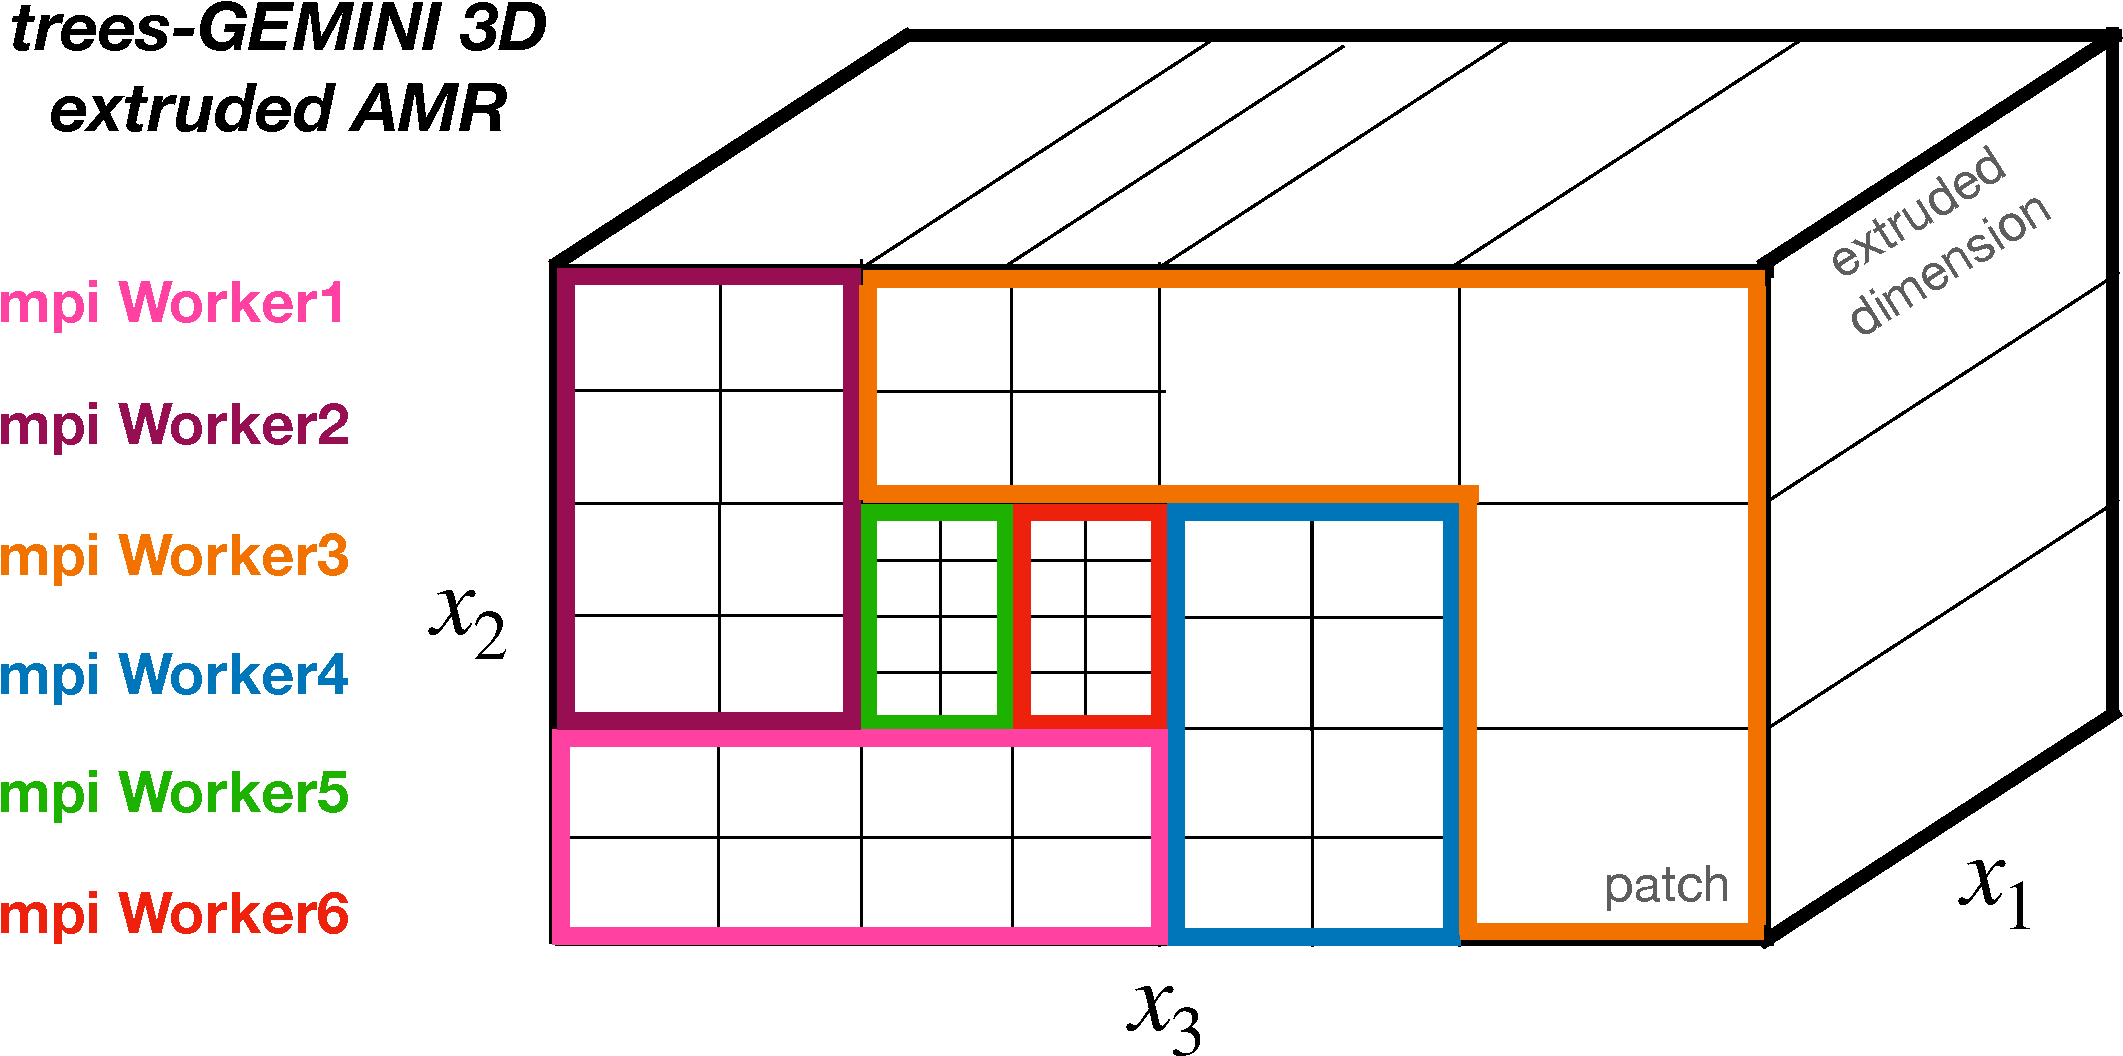
\includegraphics[width=0.8\textwidth]{./figures/GEMINI_parallel-crop.pdf}
  \caption{Trees-GEMINI use of forestclaw extruded mesh AMR and parallelization.}
  \label{fig:parallel}
\end{figure}

Trees-GEMINI currently contains most of the functionality of the core libGEMINI libraries including input data handling, dipole and Cartesian meshes, specifications of boundary conditions, fluid plasma solvers (chemistry, advection, diffusion), photoionization and impact ionization solvers, along with new output routines to optionally generate \texttt{vtk/vtu} files for efficient 3D visualization via the Paraview multi-platform open source application (Figure \ref{fig:Trees-GEMINI} shows an example).  It currently does not have a AMR-capable (quasi-static) potential solution in the manner of the core GEMINI library as this functionality was not required by the projects that funded development of Trees-GEMINI.  While the MAGIC data are historically input via files, a strategy for running the models side-by-side and exchanging data (one-way) thru memory is currently in development and testing as part of AtmoSense in a form that can, next, be reciprocated from GEMINI to MAGIC.  %Two-way GEMINI-MAGIC communication is not part of any currently funded project and will be needed for the proposed studies.  

Figure \ref{fig:Trees-GEMINI} shows a Trees-GEMINI simulation using multiply refined regions to model low-frequency acoustic wave propagation through the ionosphere using input from the MAGIC atmospheric dynamics model.  
\begin{figure}
  \includegraphics[width=\textwidth]{./figures/allGEMINI-crop.pdf}
  \caption{Trees-GEMINI simulation of mHz acoustic waves (AWs) propagating through the ionosphere using input data from MAGIC.  (a,b) The overall grid and refinement structures used in the simulation, (c) the configuration of plasma flow, (d) individual output frame illustrating how AW forces ion flows in the F-region and topside.}
  \label{fig:Trees-GEMINI}
\end{figure}


\subsection{Use of \texttt{trees-GEMINI} within the \texttt{FIGMENTS} framework}

Trees-GEMINI has been integrated with the FIGMENTS framework which uses p4est and forestclaw functions to search for overlap between two AMR meshes and to interpolate data from one mesh onto another for purposes of model coupling.  The advantage of this approach over the traditional file-based data exchange (Figure \ref{fig:org}) is that that data exchange is done in memory and during execution of both models.  As such this approach is must more efficient that the traditional interfaces and moreover allows AMR data exchange not possible in prior implementations.  
\begin{figure}
  \centering
  \includegraphics[width=0.7\textwidth]{./figures/figments-crop.pdf}
  \caption{Tree-GEMINI run within the FIGMENTS framework.  This simulation includes MAGIC-forest modeling of a source representative of the Mistry Picture Experiment which is then conveyed via forestclaw memory searches to trees-GEMINI.  Show in the diagrams are the mesh refinement in GEMINI (top) along the field-aligned component of the plasma drift velocity when forced by the shock wave.}
  \label{fig:FIGMENTS}
\end{figure}

Figure \ref{fig:FIGMENTS} shows an example of trees-GEMINI and MAGIC-forest coupled through the FIGMENTS framework.  This example uses the Misty Picture source in MAGIC-forest and the results plots show how the shock wave manifests in plasma drifts in the trees-GEMINI model.  


\section{Postprocessing and Visualization Scripts}

\emph{MH - can you fill in this section explain basic function of pygemini and mat\_gemini?}


\section{Continuous Integration (CI)}

\subsection{Automatic CI}

The base \texttt{gemini3d} repository includes a set of integration and unit tests that can be run by a user upon compilation of model to test a number of model components as well as several integration tests that run simple model configurations and compare results against reference data archived in online repositories.  These tests are also run via GitHub Actions anything a new update is pushed to the \texttt{gemini3d} repository.  These test are designed to be able to run in a matter of minutes on a modest computer.  

\emph{MH:  cmake implementation details, locations of reference data, details of github actions and examples, descriptions of tests}

\emph{MH - example plots of output?}

\subsection{Comprehensive Continuous Integration (long CI)}

Integration tests done by the automatic CI system are necessarily limited to those which can run quickly; yet there are a huge number of potential applications of the GEMINI model.  A more comprehensive set of tests, in the \texttt{gemci} repository have been developed in order to check a number of other common use cases of the model against reference data.  These include:
\begin{itemize}
  \item Instability development utilizing periodic grids and quasi-dynamic solvers:  
  \item Auroral electron precipitation and field-aligned currents:  
  \item 2D and 3D cusp, open curvilinear grids with soft electron precpitation and field-algned:   currents
  \item Closed, dipole grids with file input neutral perturbations:  
\end{itemize}
A more comlpete description of each of these tests is given in the README file in the \texttt{gemci} repository under the \texttt{cfg} folder.  The complete set of long CI tests is designed to be run in about 12 hours on a modest computer system.  

\emph{MH:  cmake implementation details, locations of ref. data}

\emph{MH - example plots of output?}



\section{Examples and Comparisons Against GNSS Data}

\emph{PI - add some of the most recent comparisons you've done during this project?  Or a reference to your section of the report?}



\pagebreak
\setcounter{page}{1}

\bibliography{../formulation/GEMINI.bib}

\end{document}
